\setlength{\parskip}{\baselineskip}
\section{Appendix}


\begin{frame}
	\huge Appendix
\end{frame}

\begin{frame}{Convolutional Neural Network}
    \begin{figure}
        \centering
        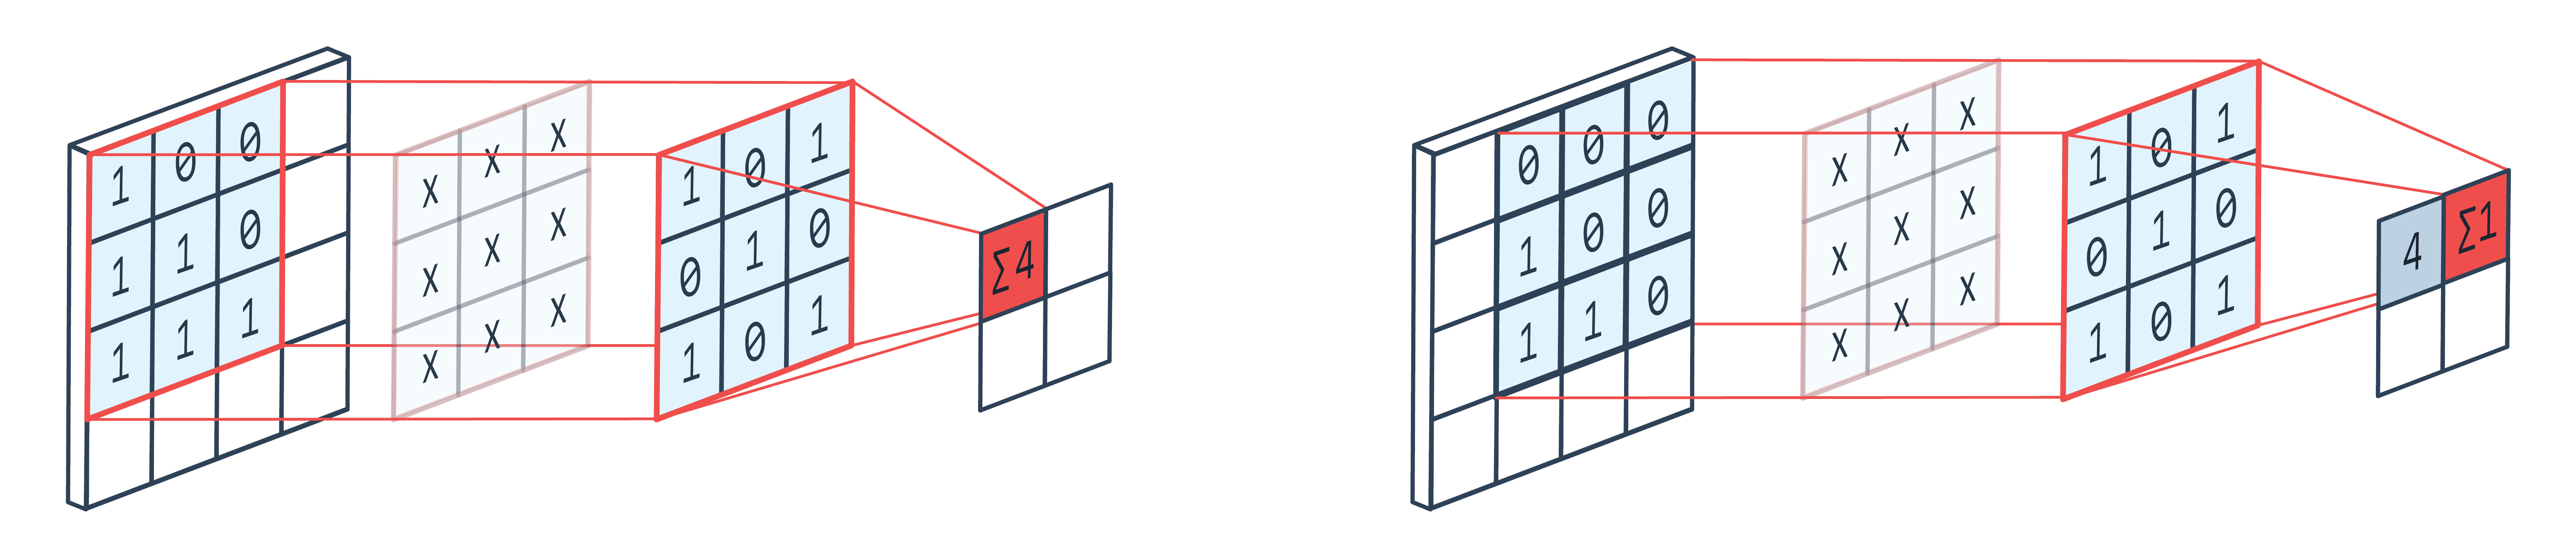
\includegraphics[height=0.25\textheight]{Images/Diagrams/2d_convolution.png}
        \caption{2D convolution}
    \end{figure}\\
    \begin{figure}
        \centering
        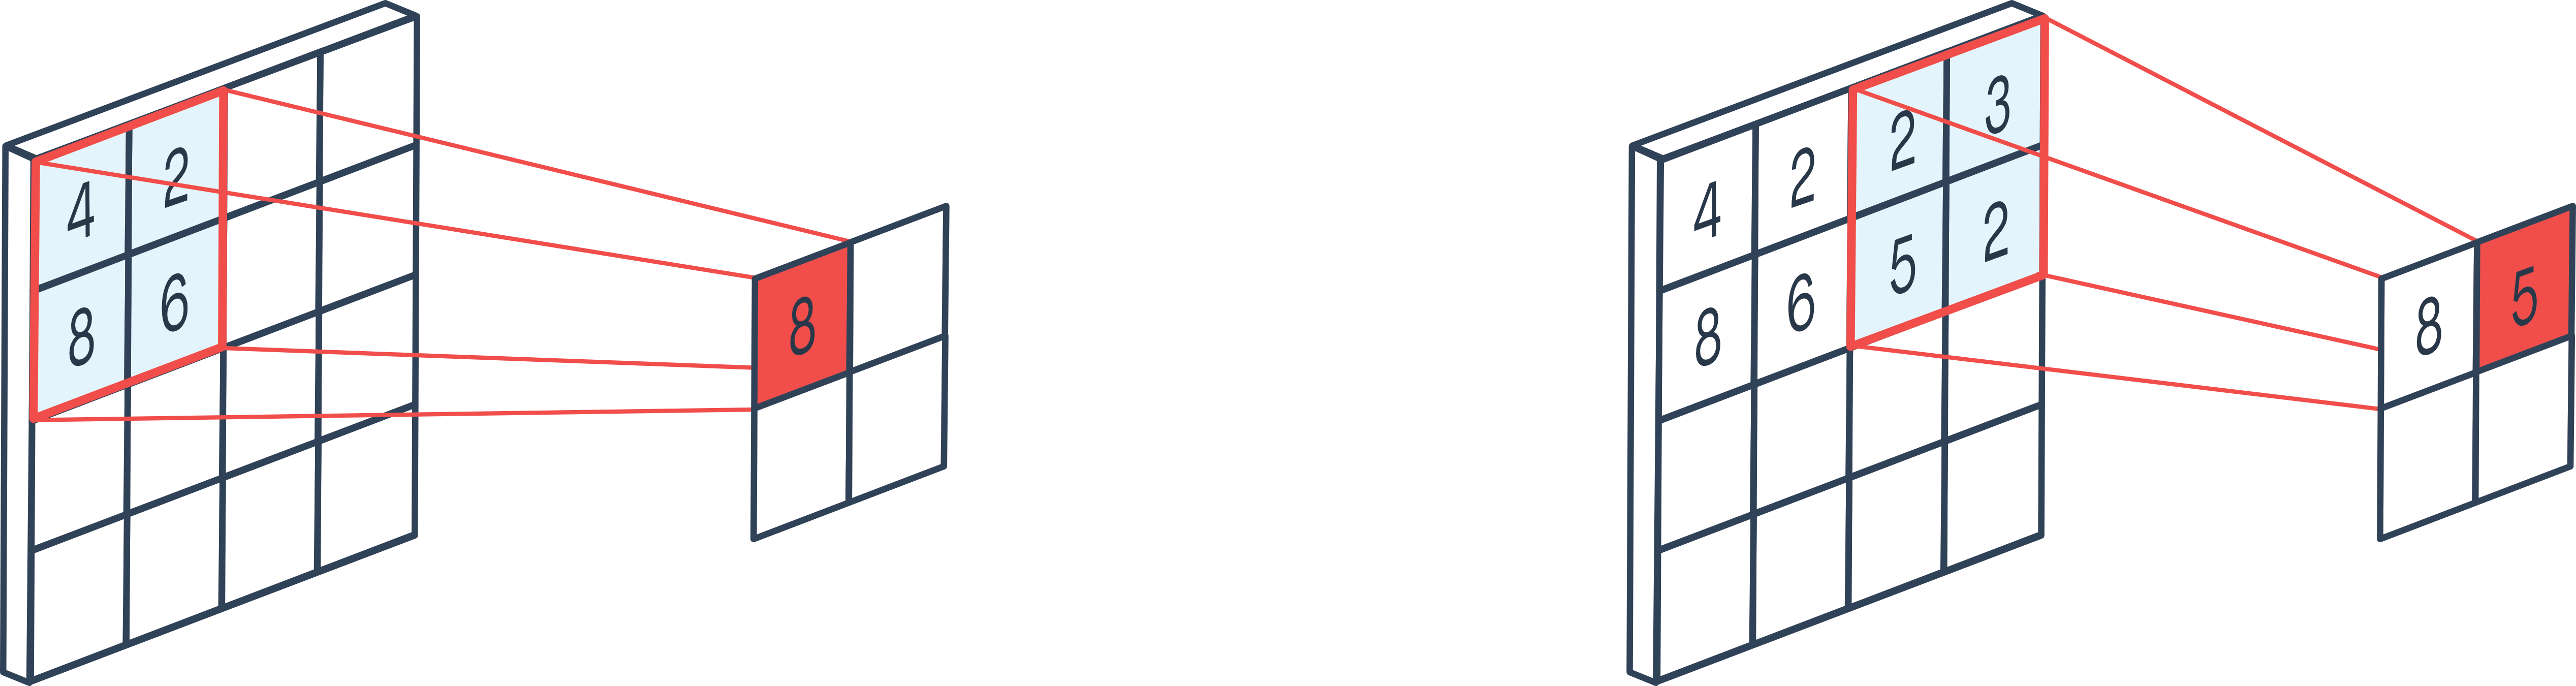
\includegraphics[height=0.2\textheight]{Images/Diagrams/2d_max_pooling.png}
        \caption{2D max pooling}
    \end{figure}%
\end{frame}

\begin{frame}{FL Algorithms}
   Distributed SGD\\
    \begin{itemize}
        \item initially intended for training in datacenters
        \item workers compute new models from distinct mini-batches in parallel
        \item synchronization service aggregates workers' models
        \item can be generalized for FL, referred as Federated SGD
    \end{itemize}
    FederatedAveraging\\
    \begin{itemize}
        \item Cornerstone of FL, most FL algorithms are its derivatives
        \item clients compute new models from distinct datasets in parallel
        \item server aggregates clients' models
        \item each GE, local datasets are split in batches and exhausted completely
    \end{itemize}%
\end{frame}

\begin{frame}{Thesis Approach}
Many components, requiring different development tools.
Split the development in distinct steps.\\
	\begin{enumerate}
	    \item develop the synchronization \& communication parts of the FL system
	    \item implement local training using TensorFlow
	    \item explore the behaviour of the complete FL system
	    \item create an optimized FPGA-based CNN training accelerator
	    \item merge the FPGA-based accelerator with the FL system
	\end{enumerate}
\end{frame}

\begin{frame}{FPGA-based CNN implementation - 2D Convolutional Layers - Forward Propagation}
	\begin{minipage}{0.4\textwidth}
    	\begin{figure}[H]
            \centering
    		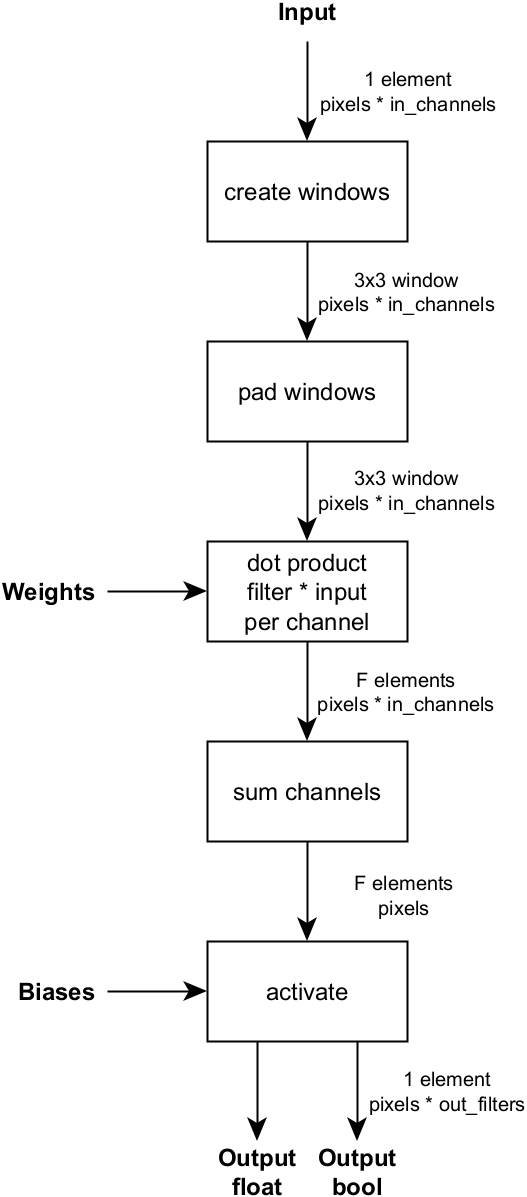
\includegraphics[height=0.65\textheight]{Images/Diagrams/conv2d_fp_mc.png}
            \caption*{Conv2D: Forward Propagation}
    	\end{figure}%
	\end{minipage}%
	\begin{minipage}{0.6\textwidth}
    	\begin{itemize}
    	    \item Inputs and outputs are streamed serially to maintain compatibility with other layers
    	    \item Internal streams are more flexible
    	    \item Filters are calculated in parallel
    	\end{itemize}
	\end{minipage}%
\end{frame}

\begin{frame}{FPGA-based CNN implementation - 2D Convolutional Layers - Back Propagation \& Gradient Calculation}
	\begin{minipage}{0.4\textwidth}
    	\begin{figure}[H]
            \centering
    		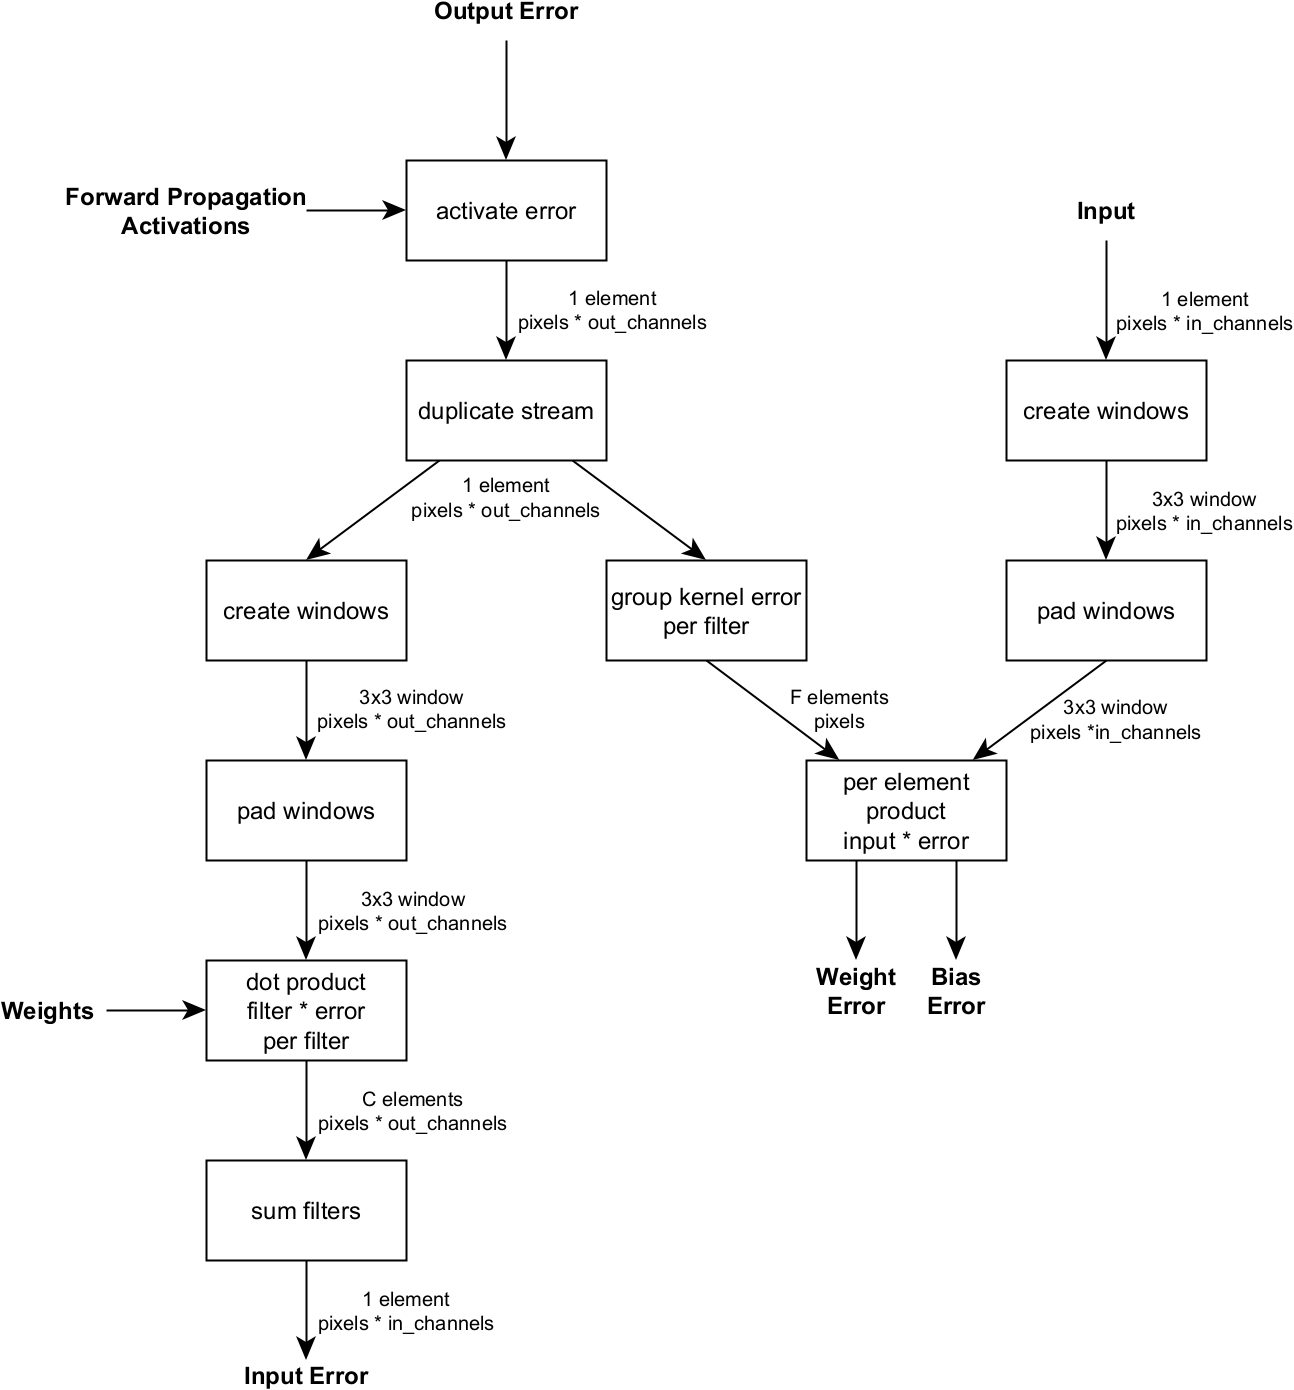
\includegraphics[height=0.7\textheight]{Images/Diagrams/conv2d_bp_cg_mc.png}
            \caption*{Conv2D: Back Propagation}
    	\end{figure}%
	\end{minipage}%
	\begin{minipage}{0.6\textwidth}
    	\begin{itemize}
    	    \item ReLU activate the error
    	    \item Compared to forward propagation, filters and input channels exchange places
    	\end{itemize}
	\end{minipage}%
\end{frame}

\begin{frame}{FPGA-based CNN implementation - 2D Max Pooling Layers - Line Buffers}
	\begin{minipage}{0.5\textwidth}
    	\begin{figure}[H]
            \centering
    		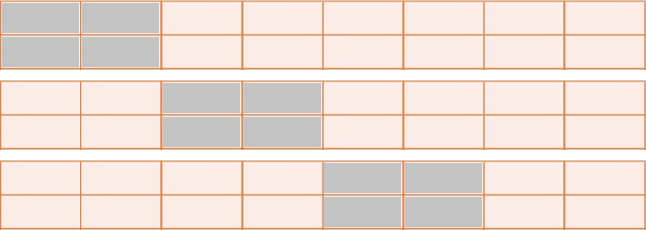
\includegraphics[width=1\textwidth]{Images/Diagrams/maxp_accesss_patern.png}
            \caption*{Line Buffers with 2$\times$2 windows and stride 2}
    	\end{figure}%
	\end{minipage}%
	\begin{minipage}{0.5\textwidth}
    	\begin{itemize}
        	\item Write input pixels serially
            \item Access them through sliding 2$\times$2 windows with stride 2
            \item Padding is not required
    	    \item Expandable for multiple input channels
    	    \item After that, only a comparison is required
    	\end{itemize}
	\end{minipage}%
\end{frame}

\begin{frame}{FPGA-based CNN implementation - Data Movement \& Storage}
    The majority of data movements are implemented with FIFOs. Implementation provided by the Vitis HLS "hls\_stream.h" library. % pipelines are designed around them
    
    FIFOs that skip layers require a depth of 1.5-2$\times$ the data that are produced by a single image.
    
    Weights, biases, gradients and momenta are stored in BRAM. The models in Global Memory are accessed only at the start \& finish of the accelerator's operation. % ola ta dedomena pou exoun diarkia zwhs panw apo mia epanalipsh enos pipeline, apo8ukeuontai on-chip sthn BRAM
    
    Images and labels are always read from Global Memory. Images are stored twice so they can be easily accessed as required by the gradients calculation pipeline.
\end{frame}


\begin{frame}{FPGA Implementation Analysis - Resource Utilization Analysis}
    Float32 accuracy, back-propagation and SGD with momentum increase utilization considerably, even for such a small CNN.
    \begin{table}[H]
        \center
        \begin{tabular}
            { | l | r | r | r | }
            \hline
            Resource & Utilization & Available & Utilization \%\\
            \hline
            LUT      & 161274 & 274080 & 58.84\\
            LUTRAM   &  14270 & 144000 &  9.91\\
            FF       & 260050 & 548160 & 47.44\\
            BRAM     &    573 &    912 & 62.83\\
            DSP      &    854 &   2520 & 33.89\\
            \hline
        \end{tabular}
        \caption*{Post place \& route resource utilization.}
    \end{table}
\end{frame}